%!TEX root = ../main.tex

\section{Electronics Design}
\label{sec:electronics}
\todo[inline]{We should have a very broad introduction somewhere. With diagrams of all the electric board. We should write somewhere that we chose the 3-phase driver and why.  - Mikkel.}

This section is dedicated to describing the electronics designed throughout this report.
This includes an analog, a digital and a power board, as well as a driver board.
Each of these boards, the choice of components and the layout will be discussed in appropriate detail in the following sections.
One aspect of the layout specifically is important; the grounding layout.
As this discussion provides a convenient means of giving an overview of the various components, the grounding will be discussed initially:

\subsection{Electronics Components and Ground Layout}
\todo{Thomas: Someone needs to verify/elaborate on my claims about noise below}
As previously mentioned, there are four boards in this design.
Across these four boards are three different ground planes: digital ground (GNDD), analog ground (GNDA) and power ground (GNDP).
Keeping these seperate is done mainly to avoid noise propagating throughout the circuits.
For instance, GNDP is used as the return path of the high currents flowing through the motor.
The voltage on this rail is likely to be fluctuating significantly.
This will surely compromise the integrity of more crucial signals such as the current measurements used to determine the position of the rotor.
GNDD will also carry significant noise from the digital circuitry and should also be kept separate from GNDA.
The only crossover between the GNDD and GNDA will happen in the DRV8301DCA (see section \ref{sec:driverboard}) and in the NOR circuitry described in section \ref{sec:nor}.
The latter occurs at the over-current event signal which is generated on the analog board but used in the digital system.
An analog signal is fed to the SN74LVC1G17, a buffer with built-in Schmitt-trigger circuitry which is supplied from the digital 3.3$V$ rail.\\
A simplified overview of the grounding planes can be seen on figure \ref{fig:groundplanes}.

\begin{figure}[!h]
	\centering
	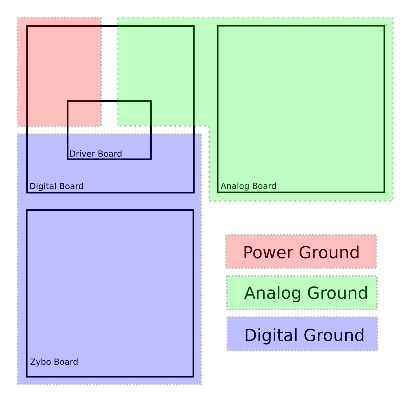
\includegraphics{graphics/ground_plane}
	\caption{Simplified view of the electronics with the ground planes marked.}
	\label{fig:groundplanes}
\end{figure}

As it is undesirable to have the potentially noisy GNDP present on the boards, it is constrained to one corner of the digital board.
Here it is used to supply the TEN20-4823WIN and the TVN5-4811WI isolated dc-dc converters that generate the $\pm15V$ and $5V$ rails respectively.
The previously mentioned 3.3$V$ rail is generated on the Zybo board.
The driver chip (The DRV8301DCA is discussed in more detail in section \ref{sec:driverboard}), is also supplied from the power rail, and as such GNDP is extended to a corner of the driver board.
Limiting the extent of GNDP is also the reasoning behind generating the $\pm15V$ rail on the digital board, even though it is used exclusively on the analog board.
An extended discussion of the grounding planes as well as the actual layout can be found in appendix

\subsection{Analog Board}
The analog board houses, as the name implies, all of the analog signal processing.
Mainly the over-current protection, but also the torque pedal scaling is present on this board.

\subsubsection{Over-current Protection}
In order to protect the system, it is necessary to create some form of over-current protection, OCP.
Three choices immediately present themselves:
\begin{enumerate}
	\item The DRV8301 is equipped with current sensing circuitry that allows the chip to automatically shut down the drivers when an over-current event, OCE, occurs.
	This requires the use of external shunt resistors to divert some of the current through the mosfets to the current sensors.
	\item Since the LF 205-S current transducers are used to measure the current through each of the phases, these measurements could be scaled such that they fulfil the role of the shunt resistors, still utilizing the built-in OCP of the DRV8301.
	\item Build circuitry that, based on the measurements done by the current transducers, detects an OCE and turns off the drive signals. 
\end{enumerate}
Initially 2 seemed like a sensible choice, however it was not possible to deduce the functionality of the OCP in the DRV8301 based on the datasheet.
Therefore it was decided to use 3 since the function will be well known and can be easily adjusted to meet any altered requirements, should the need arise.\\

Since only two phases are measured directly it is necessary to calculate the third.
This is done using a non-inverting summing amplifier.
See figure \ref{fig:sumamp}.
The output of this amplifier is given by:
\begin{equation}
	V_{out} = \left(1+\frac{R_4}{R_3}\right)\left(V_1\frac{R_2}{R_1+R_2}+V_2\frac{R_1}{R_2+R_1}\right)
\end{equation}

No amplification of the signals is wanted, thus the resistances are all set to $R=20k\Omega$. \todo{Thomas:Need correct values from Klaus/Martin}
With all three phase signals available it is possible to process them to detect any OCE's. 

\begin{figure}
	\centering
	\noindent\makebox[\textwidth]{\includegraphics[width=2\linewidth, trim=0cm 9cm 0cm 8cm]{graphics/sumamp}}
	\caption{The non-inverting summing amplifier used to calculate the current in the third phase.}
	\label{fig:sumamp}
\end{figure}

\begin{figure}
	\centering
	\includegraphics[width=\linewidth, trim=0cm 6cm 0cm 5cm]{graphics/ocp_phase}
	\caption{One phase of the over-current protection circuit.}
	\label{fig:ocpcircuit}
\end{figure}

The entire protection circuit for one phase can be seen in figure \ref{fig:ocpcircuit}.
Here the circuit has been split in accordance with the functionality of its four main parts: ADC isolation, full wave rectifier, thresholding circuit and an inverter.
Each part will be explained in appropriate detail in the following paragraphs.

\paragraph{ADC Isolation:}
The current measured in each phase is used in the control of the motor and as such it is important to maintain the integrity of the signal.
Therefore, after routing the signal to the ADC it is applied to the OCP circuit through a voltage follower.
Since the op amp has extremely high input resistance ($10^{12}\Omega$ in the case of the LF353 used in this circuit) what happens on the output-side of the voltage follower has no meaningful impact on the input-side.

\paragraph{Full Wave Rectifier:}
The phase signals are sinusoids with an expected peak amplitude of $\pm0.5V$.
In order to only needing to detect a positive OCE the signal is rectified.
Due to the small magnitude of the signals it is necessary to use a precision full wave rectifier.
The rectifier used here can be divided into two subcircuits; a half-wave rectifier and a summing amplifier.
In order to show the functionality of the rectifier, three test points are marked on the circuit, $V_i$, $V_r$, and $V_o$.
$V_i$ is the input voltage, $V_r$ is the rectification stage and $V_o$ is the rectified signal.
Figure \ref{fig:rectifier} shows the voltages at these points.

\begin{figure}
	\centering
	\includegraphics[width=\linewidth]{graphics/rectifier}
	\caption{The condition of the signal at points $V_i$, $V_r$ and $V_o$ in the full wave rectifier.}
	\label{fig:rectifier}
\end{figure}



\paragraph{Thresholding:}
As explained in section \ref{sec:lemsensor}, the input signal to the OCP circuit is dimensioned such that the maximum current in either of the phases will result in a voltage of 0.5$V$.
Also mentioned in this section is the desire to leave some headroom in case of an OCE.
This is due to the response time of the system.
50$mV$ is estimated to be sufficient.
An OCE is therefore defined as a time where the voltage exceeds 0.45$V$.
In order to avoid repeatedly switching the signal on and off, it was decided to use a Schmitt trigger.
Determining the component values is done using the following equations:

\begin{align}
	\frac{V_{cc}-V_h}{R_{7}}&=\frac{V_h}{R_8}+\frac{V_h-V_{ref}}{R_6} \label{eq:vhigh}\\
	\frac{V_{dd}-V_l}{R_{7}}&=\frac{V_l}{R_8}+\frac{V_l-V_{ref}}{R_6} \label{eq:vlow}
\end{align}

Where $V_{ref}=2.5V$ as set by the LM4040\footnote{Precision 2.5$V$ voltage reference}, the supply voltage $V_{cc}=15V$.
The desired hysteresis voltages $V_h$ and $V_l$ are $0.475V$ and $0.25V$ respectively.
This ensures that the enable signal will be pulled low when the current through any of the phases exceeds 285$A$, and will not return until the current is below 150$A$.
The LM4040 supplies a voltage in, effectively the same manner as a linear voltage supply.
It is therefore desirable to draw as little current from the component, that is, through $R_6$, as possible.
As per the datasheet it can operate from 60$\mu A\rightarrow15mA$.
It was decided to set the maximum current through $R_6$, $\frac{V_{ref}-V_l}{R_6} = I_{R_6}=100\mu A$.
This sets $R_6 = 22.5k\Omega$.
$R_7$ and $R_8$ can now be isolated using \ref{eq:vhigh} and \ref{eq:vlow}:

\begin{align}
	R_7 &= \frac{(V_{cc}V_l-V_{dd}V_h)(V_l-V_{ref})}{I_{R_6}(V_h-V_l)V_{ref}}\label{eq:r7}\\
	R_8 &= \frac{(V_{cc}V_l-V_{dd}V_h)(V_l-V_{ref})}{I_{R_6}(V_{cc}(V_l-V_{ref})-V_{dd}(V_h-V_{ref})+(V_h-V_l)V_{ref})}\label{eq:r8}
\end{align}

Resulting in $R_7 = 150k\Omega$ and $R_8 = 2542.37\Omega$.
Since 2542.37$\Omega$ is hardly a standard value, the nearest standard value is chosen such that $R_8=2550\Omega$.

\paragraph{Inverter:}
Due to the NOR-stage described in section \ref{sec:nor}, it is necessary to invert the signal.
A simple comparator is used to achieve this effect.
The input voltage to this stage is either $V_{cc}$ or $GNDD$, the voltage on the non-inverting terminal is therefore not critical.
Setting $R_9=R_{10}=10k\Omega$ is sufficient.

The circuitry discussed above will ensure that in case of an OCE, a signal is sent to the digital board where it will be used to safely handle the event.
This is discussed in further detail in later sections. 

\subsubsection{Current Transducer - LF 205-S}
\label{sec:lemsensor}
While these current sensors are not strictly part of the analog board, the circuitry related to them is and therefore it was chosen to include their description here.
The LF 205-S utilises the Hall effect in order to measure the current flowing through a wire.
Figure \ref{fig:lf205function} depicts an equivalent circuit of the functionality of the transducer.
As can be seen, the LF 205-S functions like a transformer.
As per the datasheet this transformer has a 1:2000 turns ratio, therefore the secondary current, $I_S$ can be found as:
\begin{equation}
	\frac{I_S}{I_P}=\frac{N_P}{N_S} \quad \Rightarrow \quad I_S = \frac{I_P}{N_S}
\end{equation}
Essentially, the LF 205-S generates a current proportional to the current flowing through the device, the primary current; $I_P$.
By changing the value of the resistor $R_m$, the resulting voltage drop can be dictated.

In section \todo[inline]{Thomas: Section documenting the maximum current to be expected in each phase.} the maximum current to be expected in each phase is found to be 300$A$.
As described in section \todo[inline]{Thomas: section on the zybo adc}, the ADC on the Zynq chip can work on signals in the ranges 0$V$-1$V$ or $\pm0.5V$.
Since the current is sinusoidal it can be negative.
Choosing the range $\pm0.5V$ therefore simplifies the circuitry needed to read the value correctly.
Consequently $R_m$ needs to be set such that the maximum expected current results in the maximum allowed voltage.
However, it is desirable to leave some headroom in case of an OCE, 50$mV$ should be sufficient.
Thus:
\begin{equation}
	R_m = \frac{0.45}{I_{Pmax}/N_S} = 3\Omega
\end{equation}

\subsubsection{Torque Pedal Downscale}
The torque pedal is simply a variable resistor, $R_{tp}=7.5k\Omega$. \todo[inline]{Thomas: Verify resistor value on final system}
As the pedal is actuated the resistance changes.
Figure \ref{fig:torquepedaldownscale} is a depiction of the circuit used to read the position of the torque pedal.
$R_1$ and $\mathrm{R_P}$ form a variable voltage divider of the $15V$ rail.
The analog input of the ADC in the FPGA, however, is limited to 0-1$V$.
Therefore it is necessary to downscale the voltage.
Intuitively this could be done using simply a voltage divider, but since the torque pedal functions as a voltage divider, the varying resistance distribution of the torque pedal would influence the voltage divider.
For this reason a voltage follower is used to isolate the two circuits.
In addition, a 5.1$V$ zener diode is clamping the signal to ground in order to protect the ADC of the FPGA.
\todo{capacitor for noise}
\begin{figure}[!h]
	\centering
	\includegraphics[width=.75\linewidth]{graphics/torque_pedal_downscale}
	\caption{Circuit used to scale the voltage from the torque pedal from $0V\rightarrow5V$ to $0V\rightarrow1V$.}
	\label{fig:torquepedaldownscale}
\end{figure}

The resistance of the pedal changes linearly, which means the voltage division does not. Voltage at the point TP as a function of pedal is:

\begin{equation}
V_{TP}(R_P) = V_{CC} \frac{R_P}{R1 + PEDAL} \frac{R3}{R3 + R2}
\label{eq:pedal_voltage}
\end{equation}

By isolating $\mathrm{R_P}$, it's possible to calculate what its resistance is. 
The resistance of $\mathrm{R_P}$ varies from $0$ to $7.5 k\Omega$, as the pedal is pressed down. 
Hence, equation~\ref{eq:pedal_back_calc} will give a value proportional to the torque requested by the driver

\begin{equation}
R_P = \frac{V_{TP} R1 \cdot (R2 + R3)}{R3 \cdot (V_{CC} - T_{TP}) -  V_{TP} \cdot R2}
\label{eq:pedal_back_calc}
\end{equation}

Finally, due to the mechanical nature of the torque pedal, this signal is likely to be noisy.
C$_1$ is placed in order to filter this noise.

\begin{figure}[H]
	\begin{center}
		\includegraphics[width=10cm]{graphics/pedal_voltage.pdf}
		\label{fig:pedal_voltage}
		\caption{Voltage as a function of the pedal resistance.}
	\end{center}
\end{figure}

\subsection{Digital Board}
The digital board is used mostly as an interconnection board between the various electronic components in the system.
The logic levels of the different systems are managed here along with the enable signal for the DRV8301.

\subsubsection{Drive Enable Signal}
This signal is produced by the torque pedal.
When the user actuates the pedal a switch is connected to ground. 
By reading the drive enable signal it is therefore possible to determine when the controller should be running, allowing a means for avoiding integral windup.
Since this signal is left floating when the pedal is not active, it can be routed directly to the Zybo, using the internal pull-up resistors.
\todo[inline]{Thomas: Is the torque pedal active low or active high? Correct two places above to reflect the correct case}
\subsubsection{Driver Enable Circuit}
\label{sec:nor}
The DRV8301DCA is equipped with a pin called \texttt{EN\_GATE}.
If, while running, this pin is pulled low, the drive signals are immediately shut down.
This feature allows for fast and reliable shut down of the motor in case of any detected faults.
There are two different types of faults detected within the system, the aforementioned OCE and an over-temperature event, OTE.
In addition to these two a signal is routed from the Zybo which enables the digital part of the system to disable/enable the motor, should the need arise.
As there are three different signals that all need to connect to the same pin, they are all NOR'ed, as seen in figure \ref{fig:driveenablesignal}.

\begin{figure}[!h]
	\centering
	\includegraphics[width=\linewidth,trim=0cm 3cm 0cm 3cm]{graphics/driver_enable_signal}
	\caption{The NOR circuit that compares the three enable signals to determine whether the drive signals should be on.}
	\label{fig:driveenablesignal}
\end{figure}

The observant reader will notice that two 2-input NOR gates was used rather than one 3-input gate.
Reason for this is that the OTE protection was not implemented until after the components were ordered.
In order then to not need additional components it was decided to cascade the available component.
This cascading however does mean that it is necessary to invert the logic level of the signals OCE, and OTE.
OCE is inverted on the analog board while OTE is used to pull the signal to ground.
The two signals are both routed to the Zybo.
This is done such that it is possible to discern which event has triggered when the motor halts.

\subsubsection{Logic-Level Shifters}
Tracking the angular position of the rotor is done using an encoder mounted on the motor.
Upon receiving a clock signal the encoder will return the current position of the rotor.
The encoder module is an AM256 which, according to the datasheet, requires at least 3.5$V$ for digital high input.
However, the Zybo uses 3.3$V$ and the clock signal therefore needs to be shifted to the correct voltage level, 5$V$. 
A, B, Z and Data generated by the AM256 all need to be shifted down to 3.3$V$ in order to protect the Zybo.
The circuit for these four signals can be seen in figure \ref{fig:lls}.
The buffer used for these signals is, as can be seen from the figure, the 74AHC125 which is a quad-buffer.
$V_{out}$ of this device is equal to $V_{cc}$, while $V_{in}$ can be any voltage from $0\rightarrow 5V$, by supplying it from the 3.3$V$ rail it will therefore act as a logic level shifter.

\begin{figure}[!h]
	\centering
	\includegraphics[width=.5\linewidth,trim=0cm 1cm 0cm 1cm]{graphics/lls}
	\caption[Logic level shifter circuit.]{The 74AHC125 quad-buffer used to shift the logic level of the encoder from 5$V$ down to the $3.3V$ required by the Zybo. Due to an oversight, a buffer with an enable on each port was bought. This feature is unnecessary and they are always enabled.}
	\label{fig:lls}
\end{figure}

\subsection{Driver Board}
This is not finished!
\label{sec:driverboard}

\subsubsection{SPI}
The DRV8301 is capable of performing SPI communication as a slave.
This can be used to read status registers of the chip and set configuration options.